% Provenance (never printed): cycle 2 "Questionner l'espace et le temps"
% (oceans, seas, continents on the globe) and "Questionner le monde de la
% matiere" (states of water in natural phenomena); see sources/book1/PROVENANCE.md.
% Book 1, grade 2, chapter 1.
\chapter{地球上的水}\label{ch:g2:water-on-earth}

1972 年 12 月 7 日，三位前往月球的宇航员
把照相机转向了地球。他们拍下的照片成为有史以来最著名的照片之一。
看一看这张照片。你可以看到白色的云、
一点棕色和黄色的陆地、底部白色的冰——到处都是蓝色，蓝色的。
从太空看，我们的星球是一颗蓝色的行星。

\begin{omfigure}
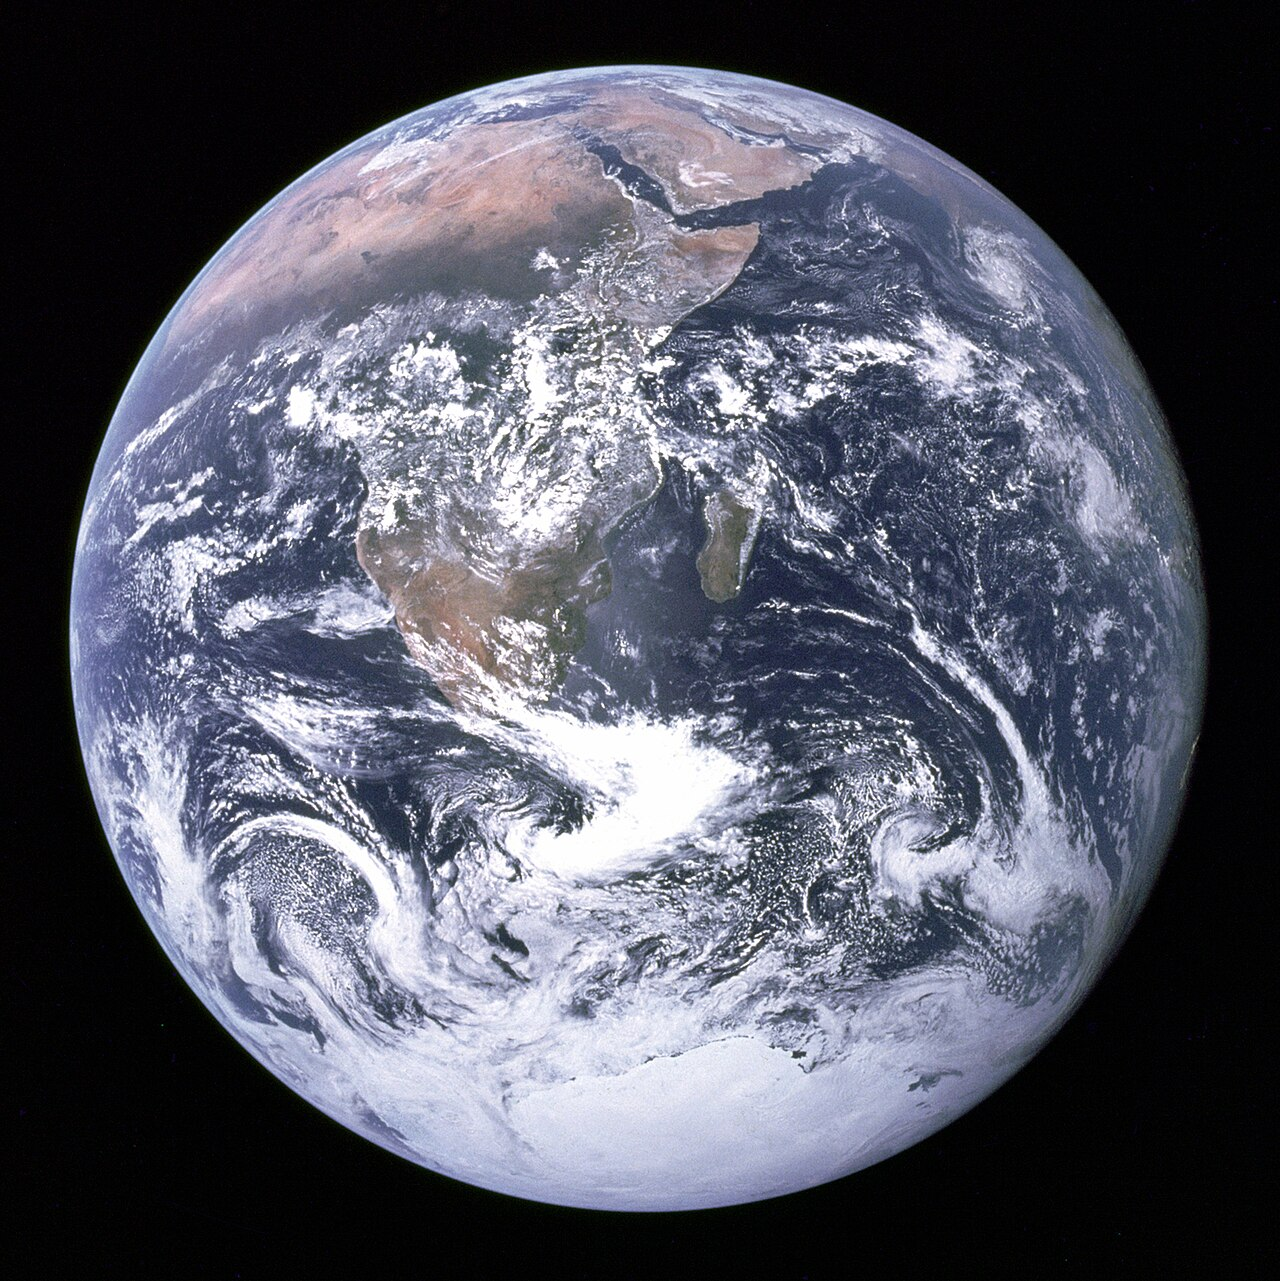
\includegraphics[width=0.5\linewidth]{images/book1/g2-nasa-blue-marble.jpg}

{\small 1972 年 12 月 7 日，阿波罗~17 号宇航员拍摄的地球。
图中可以看到非洲、上方的阿拉伯半岛，以及底部的南极洲冰原。
照片来源：NASA（公有领域）。}
\end{omfigure}

\begin{recall}
水可以是固体（冰）、液体，或者是我们看不见的气体（水蒸气）。
放在太阳下的液态水会慢慢变成水蒸气：它会蒸发。
水蒸气冷却后会变回细小的水滴：它会凝结。
这些变化你在物理书中已经见过。在\omterm{def:g1:landscapes-around-us:landscape}{景观}中，
水在\omterm{def:g1:landscapes-around-us:water}{河流}中流动，积聚在\omterm{def:g1:landscapes-around-us:water}{湖泊}里（见\cref{ch:g1:landscapes-around-us}）。
\end{recall}

\section{蓝色的星球}

地球的大部分表面被水覆盖。想象把地球的整个表面切成
100 个相等的小方格。如果把被海覆盖的每个方格涂成蓝色，
我们会涂出 71 个方格。只有 29 个方格是陆地。

\begin{omfigure}
\begin{tikzpicture}
  \begin{axis}[hide axis, width=7.2cm, height=7.2cm, xmin=-0.5, xmax=9.5,
      ymin=-0.5, ymax=9.5, axis equal image, scale only axis,
      clip=false]
    \addplot[scatter, only marks, mark=square*, mark size=9.2pt,
      scatter/classes={0={fill=green!45!omLithAlluv, draw=black!40},
                       1={fill=omSea!80!blue, draw=black!40}},
      point meta=explicit symbolic]
      table[x=col, y=row, meta=blue] {figdata/out/grade-2-ocean_fraction-grid.dat};
  \end{axis}
\end{tikzpicture}

{\small 如果把地球表面切成 100 个相等的方格，其中 71 个是海（蓝色），
29 个是陆地（绿色）。该图由全球地形图计算得出，
地形数据来自 NOAA ETOPO1。}
\label{fig:g2:water-on-earth:grid}
\end{omfigure}
% ledger: data:etopo1, wss:ocean-cover (71 % computed in figdata/grade-2/ocean_fraction.py)

覆盖地球大部分表面的大片\omterm{def:g2:water-on-earth:salt-fresh}{咸水}都有名字。

\begin{definition}[海洋和海]\label{def:g2:water-on-earth:ocean}
\emph{海洋}\index{海洋}是覆盖地球大部分表面、
位于各大洲之间的极大片\omterm{def:g2:water-on-earth:salt-fresh}{咸水}。\emph{海}\index{海}是较小的\omterm{def:g2:water-on-earth:salt-fresh}{咸水}区域，
通常位于海洋的边缘，
并部分被陆地环绕。
\end{definition}

所有\omterm{def:g2:water-on-earth:ocean}{海洋}彼此相连：船可以从任何一个\omterm{def:g2:water-on-earth:ocean}{海洋}航行到另一个\omterm{def:g2:water-on-earth:ocean}{海洋}，
而无需穿越陆地。它们的名称以及在地球仪上的位置，
见\cref{ch:g3:continents-and-oceans}。

\begin{omfigure}

\includegraphics[width=0.62\linewidth]{images/book1/ai/g2-beach-sea.jpg}

{\small 海边。海水向远方延伸，
远到眼睛看不到的地方。}
\end{omfigure}

\section{咸水和淡水}

如果你在游泳时曾咽下一口海水，你就知道：它非常咸。
\omterm{def:g1:landscapes-around-us:water}{河流}和\omterm{def:g1:landscapes-around-us:water}{湖泊}的水则不咸。

\begin{definition}[咸水和淡水]\label{def:g2:water-on-earth:salt-fresh}
\emph{咸水}\index{咸水}溶有大量盐分：它是
\omterm{def:g2:water-on-earth:ocean}{海洋}和海的水。\emph{淡水}\index{淡水}
含盐很少：它是雨水、大多数\omterm{def:g1:landscapes-around-us:water}{河流}和\omterm{def:g1:landscapes-around-us:water}{湖泊}的水，
冰雪的水，以及泉水。
\end{definition}

\begin{example}[海水有多咸？]\label{ex:g2:water-on-earth:salty}
% ledger: nos:salinity
一瓶装有 1 千克海水——约 1 升——的瓶子里，大约有 35 克盐。
如果让所有的水蒸发，盐会留在瓶底，成为白色的晶体。
海边的盐田就是这样制取海盐的：
在盐田中，太阳和风会慢慢地
把浅水池中的海水晒干。
\end{example}

\begin{omfigure}
\begin{minipage}[b]{0.49\linewidth}\centering
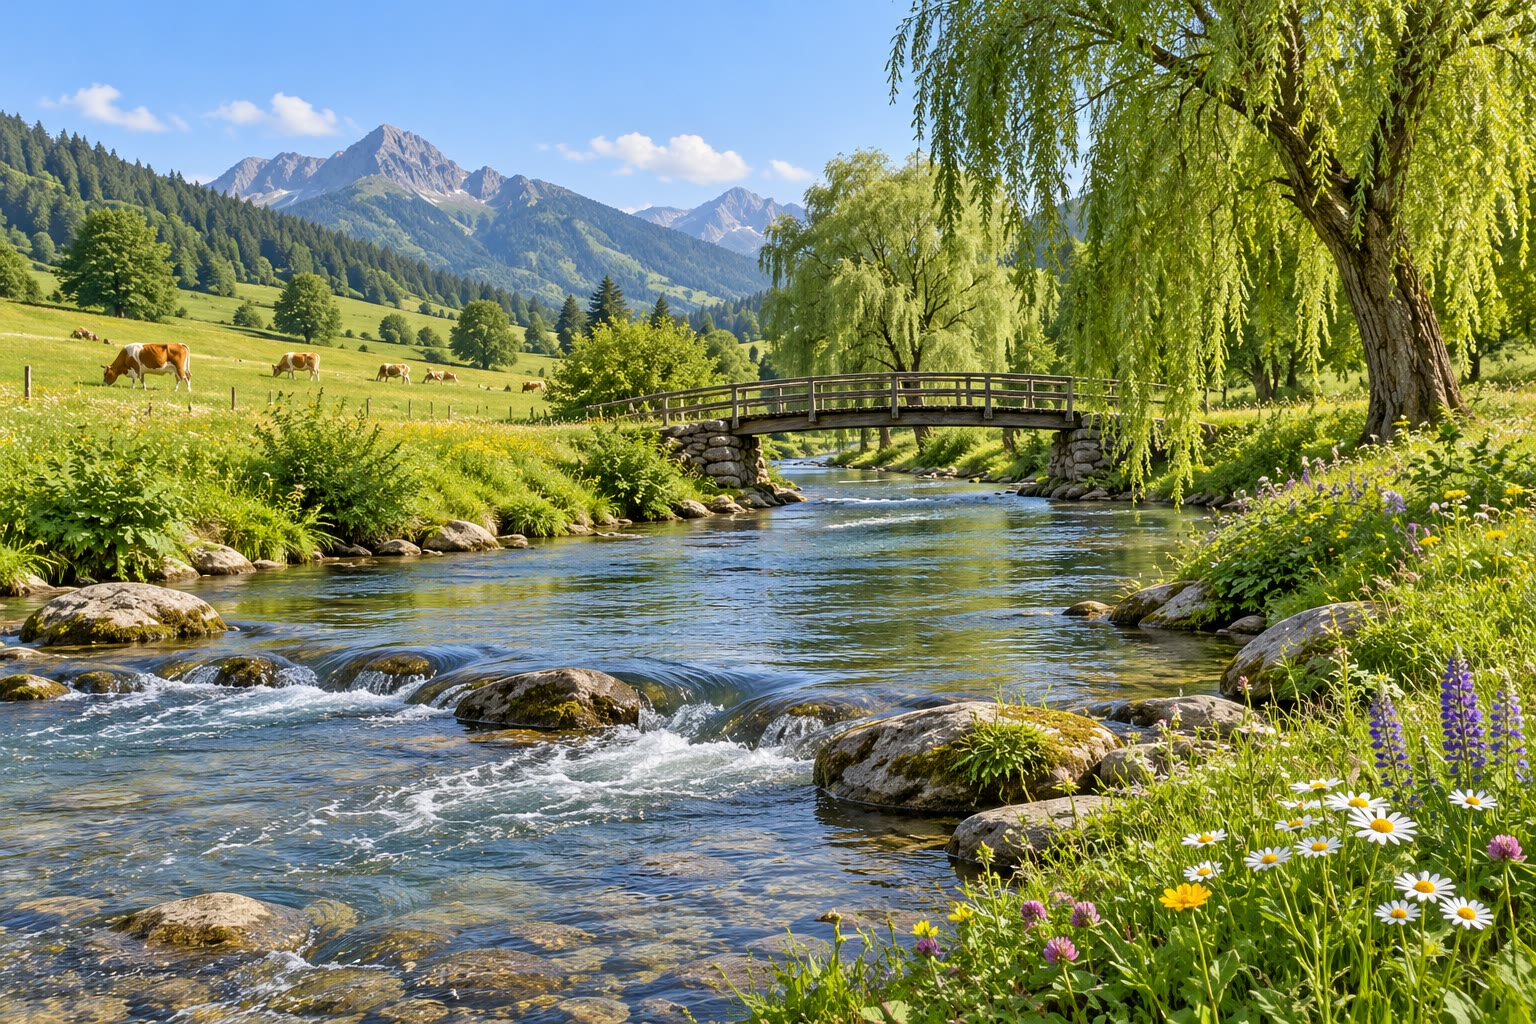
\includegraphics[width=\linewidth]{images/book1/ai/g2-river-meadow.jpg}

{\small \omterm{def:g2:water-on-earth:salt-fresh}{淡水}：\omterm{def:g1:landscapes-around-us:water}{河流}。}
\end{minipage}\hfill
\begin{minipage}[b]{0.49\linewidth}\centering
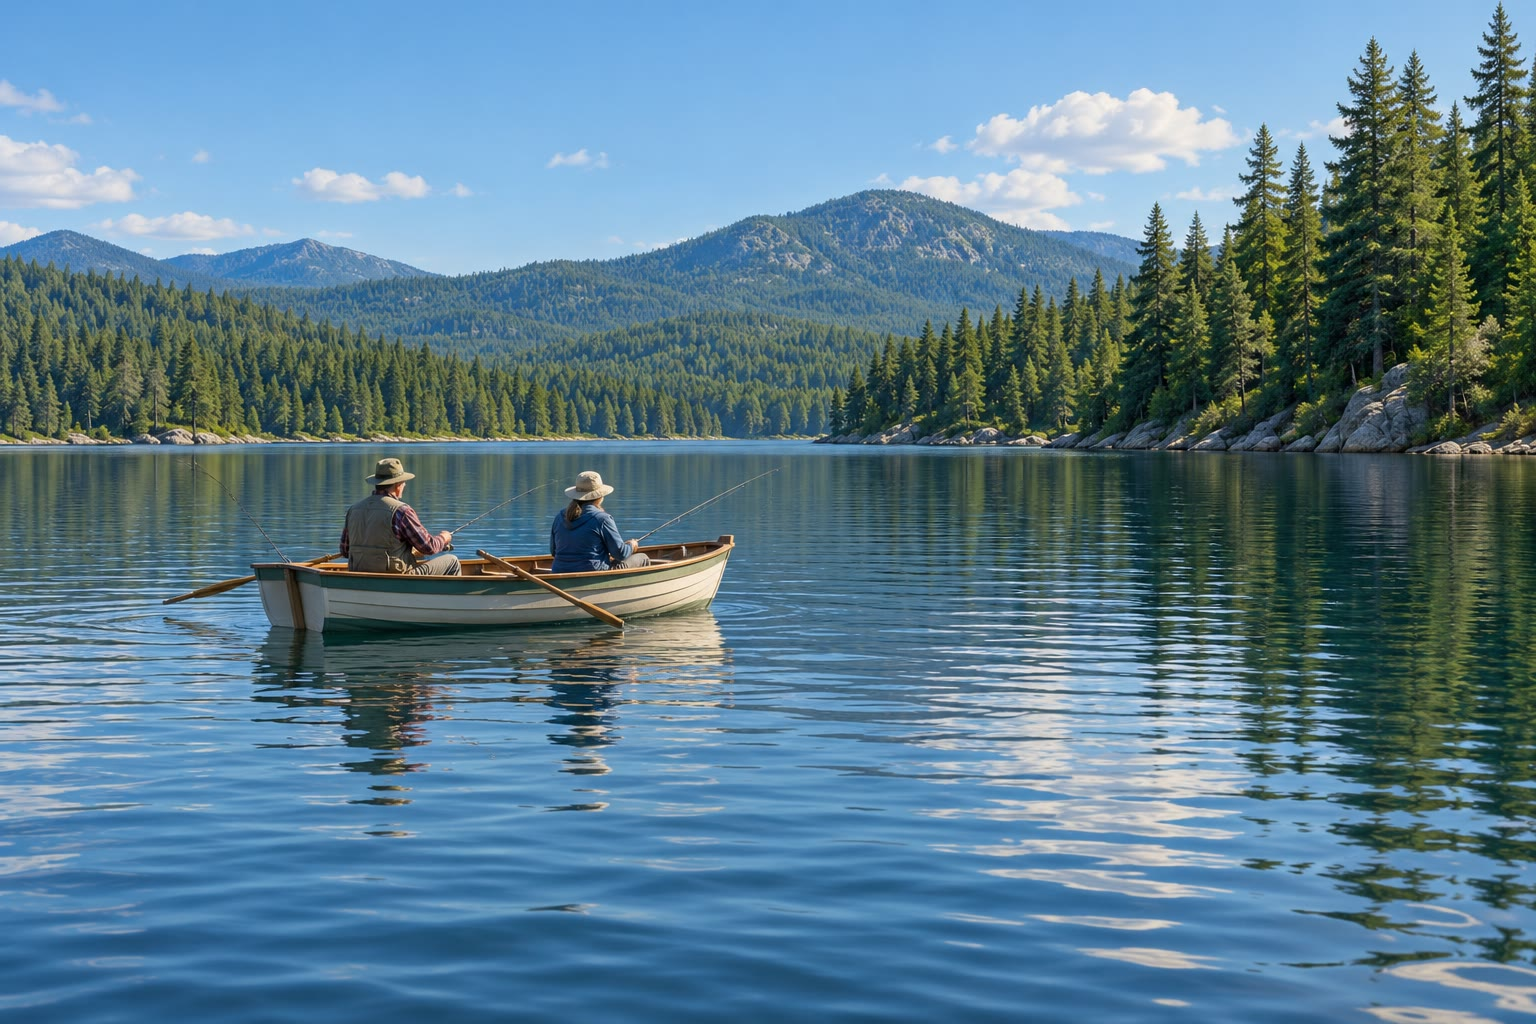
\includegraphics[width=\linewidth]{images/book1/ai/g2-lake-boat.jpg}

{\small \omterm{def:g2:water-on-earth:salt-fresh}{淡水}：\omterm{def:g1:landscapes-around-us:water}{湖泊}。}
\end{minipage}
\end{omfigure}

\begin{remark}[我们不能喝海水]\label{rem:g2:water-on-earth:drink}
人和陆地动物不能喝海水：海水中盐分太多，
喝下它会使身体失去水分，而不是获得水分。
在远离陆地、四面环水的海上，水手们一直不得不
随身携带\omterm{def:g2:water-on-earth:salt-fresh}{淡水}。
\end{remark}

\section{所有的水都在哪里？}

\omterm{def:g2:water-on-earth:salt-fresh}{淡水}不只存在于\omterm{def:g1:landscapes-around-us:water}{河流}和\omterm{def:g1:landscapes-around-us:water}{湖泊}中。很多\omterm{def:g2:water-on-earth:salt-fresh}{淡水}是冻结的：
南极洲和格陵兰岛上大片白色的冰层中，以及高山之上。
还有很多\omterm{def:g2:water-on-earth:salt-fresh}{淡水}藏在我们脚下的地下，
填满了沙粒之间细小的空隙和岩石中的裂缝。

\begin{omfigure}
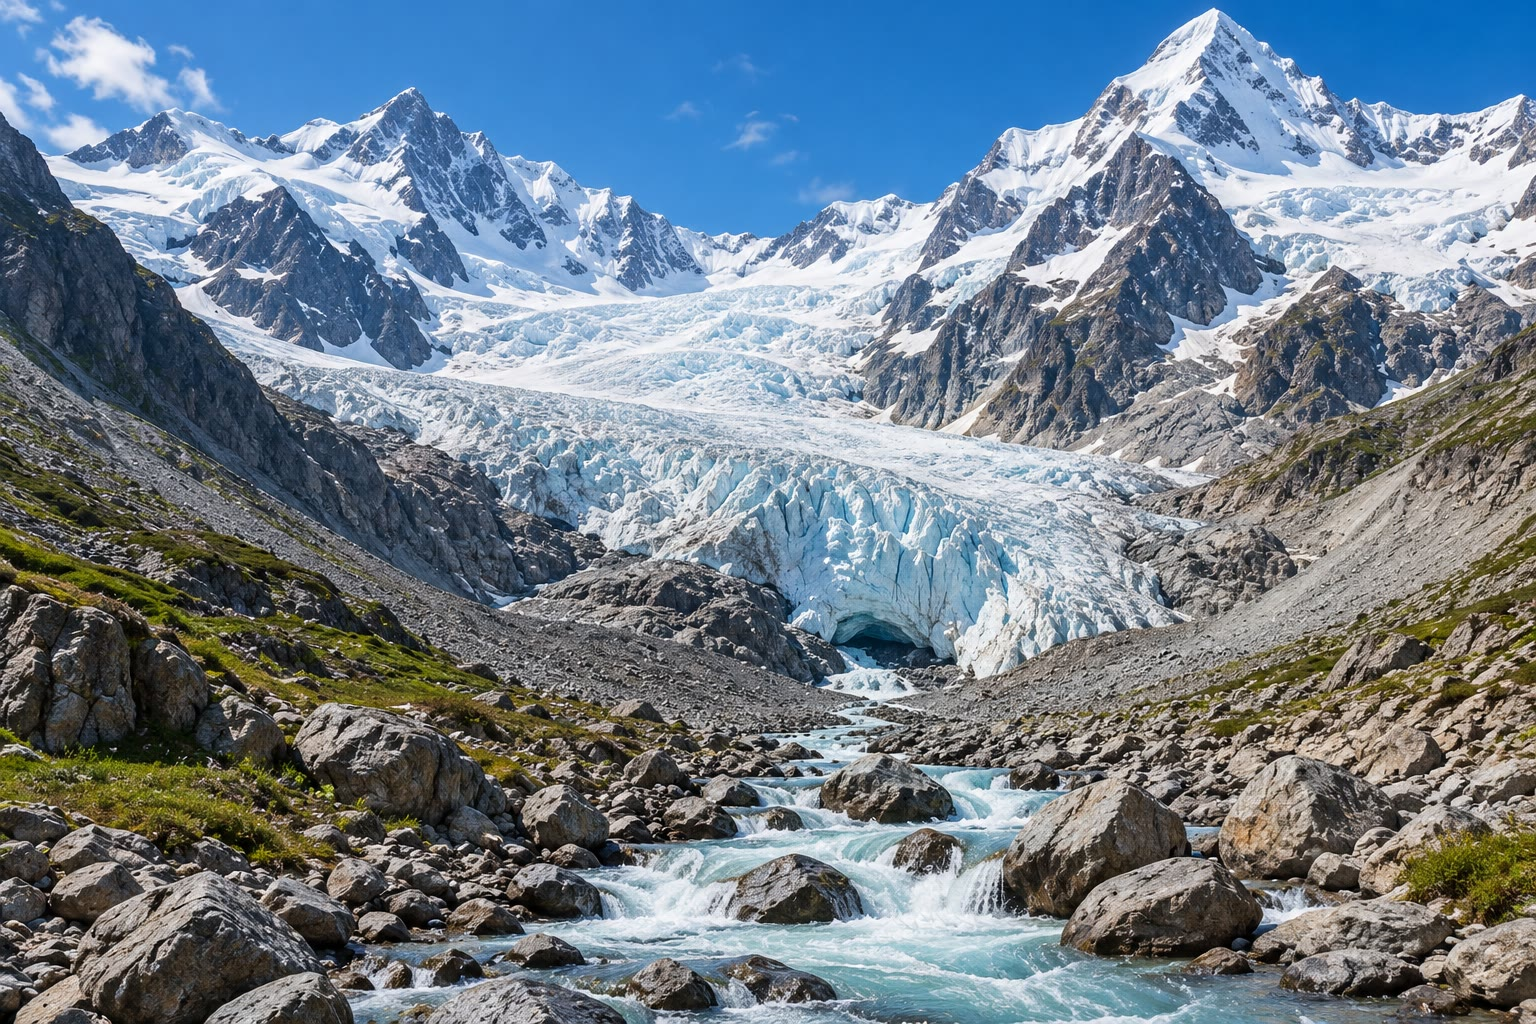
\includegraphics[width=0.62\linewidth]{images/book1/ai/g2-snowy-mountains.jpg}

{\small 高山上的\omterm{def:g2:water-on-earth:salt-fresh}{淡水}全年都以雪和冰的形式保存。在夏季，
其中一部分会融化，补给溪流。}
\end{omfigure}

想象一下，把地球上所有的水倒进 100 个大小相同的桶里。
每一类水各能装满多少个桶？

\begin{omfigure}
\begin{tikzpicture}
  \begin{axis}[hide axis, width=7.2cm, height=7.2cm, xmin=-0.5, xmax=9.5,
      ymin=-0.5, ymax=9.5, axis equal image, scale only axis, clip=false]
    \addplot[scatter, only marks, mark=*, mark size=8pt,
      scatter/classes={0={fill=omSea!80!blue, draw=black!40},
                       1={fill=white, draw=black!60},
                       2={fill=brown!55, draw=black!40}},
      point meta=explicit symbolic]
      table[x=col, y=row, meta=kind] {figdata/out/grade-2-water_shares.dat};
  \end{axis}
  \begin{scope}[shift={(7.9,5.6)}, font=\small]
    \fill[omSea!80!blue, draw=black!40] (0,0) circle (0.2);
    \node[anchor=west] at (0.35,0) {海洋中的咸水：96 个桶};
    \fill[white, draw=black!60] (0,-0.7) circle (0.2);
    \node[anchor=west] at (0.35,-0.7) {冰和雪：2 个桶};
    \fill[brown!55, draw=black!40] (0,-1.4) circle (0.2);
    \node[anchor=west] at (0.35,-1.4) {地下水：2 个桶};
  \end{scope}
\end{tikzpicture}

{\small 地球上所有的水装在 100 个桶里。\omterm{def:g1:landscapes-around-us:water}{河流}、\omterm{def:g1:landscapes-around-us:water}{湖泊}、
云和所有生物体内的水加在一起，
也装不满一个桶。数据来自美国地质调查局。}
\label{fig:g2:water-on-earth:buckets}
\end{omfigure}
% ledger: wss:water-shares (rounded to 100 buckets in figdata/grade-2/water_shares.py)

\begin{proposition}[地球上的大部分水是咸的]\label{prop:g2:water-on-earth:most-salty}
% ledger: wss:water-shares
在地球上所有水的 100 个桶中，96 个桶装的是\omterm{def:g2:water-on-earth:ocean}{海洋}中的\omterm{def:g2:water-on-earth:salt-fresh}{咸水}。
我们饮用的\omterm{def:g2:water-on-earth:salt-fresh}{淡水}只占全部水量中很小的一部分：
其中大部分被冻结在冰中，或藏在地下。
\end{proposition}

\section{雨水去哪儿了？}

下雨时，雨水不会停留在落下的地方。
雨后去看看学校的院子：一部分水顺着地面流进排水沟，
一部分渗进花坛的土壤里，
太阳重新出来后，积水会慢慢消失。

\begin{omfigure}
\begin{tikzpicture}[x=1cm, y=1cm, font=\small]
  % sky, sea, land
  \fill[ocBlue!6] (0,0) rectangle (12,5.6);
  \fill[omSea] (8.6,0) rectangle (12,0.9);
  \fill[green!30!omLithAlluv] (0,0) -- (0,2.4) .. controls (2,2.6) and (3,2.0) .. (4.5,1.6)
     .. controls (6,1.2) and (7.5,1.0) .. (8.6,0.9) -- (8.6,0) -- cycle;
  % ground below the surface
  \fill[brown!25] (0,0) rectangle (8.6,0.6);
  % river
  \draw[omSea!70!blue, line width=2.4pt] (1.6,2.45) .. controls (3.5,2.0) and (6,1.15) .. (8.6,0.95);
  % cloud and rain
  \pic at (2.2,4.0) {puffycloud};
  \foreach \x in {1.4,1.8,2.2,2.6,3.0}
    \draw[omWxRain, line width=0.8pt] (\x,3.7) -- (\x-0.15,3.1);
  \pic at (9.6,4.3) {puffycloud};
  % arrows
  \draw[omWxRain, line width=1.1pt, -{Stealth[length=2.5mm]}] (3.3,2.15) -- (3.3,0.6);
   \node[anchor=west, align=left, font=\scriptsize] at (3.4,1.0) {一部分渗入 \\地下};
  \draw[omWxRain, line width=1.1pt, -{Stealth[length=2.5mm]}] (5.4,1.55) -- (7.6,1.15);
    \node[align=center, font=\scriptsize] at (6.2,2.05) {一部分流入河流，\\河流再流入大海};
  \draw[black!50, line width=1.1pt, densely dashed, -{Stealth[length=2.5mm]}] (10.2,1.1) .. controls (10.4,2.4) and (10.1,3.2) .. (9.8,3.85);
    \node[align=left, anchor=west, font=\scriptsize] at (10.45,2.4) {水 \\蒸发};
  \draw[black!50, line width=1.1pt, densely dashed, -{Stealth[length=2.5mm]}] (8.45,4.35) -- (3.6,4.3);
  \node[font=\scriptsize, above] at (6.0,4.35) {风推动云移动};
  \node[font=\scriptsize] at (10.4,0.45) {海};
  \node[font=\scriptsize, anchor=west] at (0.2,3.25) {雨};
\end{tikzpicture}

{\small 雨水的去向。从\omterm{def:g2:water-on-earth:ocean}{海洋}和陆地上以蒸气形式升起的水
形成新的云，云又带来新的雨。}
\label{fig:g2:water-on-earth:rain}
\end{omfigure}

\begin{method}[追踪一滴雨水]\label{met:g2:water-on-earth:drop}
要追踪一滴雨水，请依次回答三个问题：
\begin{enumerate}
  \item 它落在哪里：海上、屋顶上、土壤上，
        还是山上？
  \item 它是渗入地下、沿地表流走，还是
        结成冰？
  \item 接下来它会去哪里：流入\omterm{def:g1:landscapes-around-us:water}{河流}、\omterm{def:g1:landscapes-around-us:water}{湖泊}、大海、地下，
        还是重新回到空中？
\end{enumerate}
最后，每一滴水都会回到\omterm{def:g2:water-on-earth:ocean}{海洋}或空中，
这段旅程又重新开始。
\end{method}

\begin{example}[一滴落在山上的雨水]\label{ex:g2:water-on-earth:mountain}
一滴雨水在冬天以雪的形式落在高山上。它留在那里，
冻结不动，直到夏天温暖的日子到来。然后它融化，
流入山间溪流，汇入\omterm{def:g1:landscapes-around-us:water}{河流}，再由\omterm{def:g1:landscapes-around-us:water}{河流}带到大海。
在一个晴朗的日子，这滴水从海面蒸发，升入空中，
成为一朵新云的一部分。
\end{example}

\section{练习}

\begin{exercise}[$\star$]\label{exo:g2:water-on-earth:1}
\omterm{def:g2:water-on-earth:salt-fresh}{咸水}还是\omterm{def:g2:water-on-earth:salt-fresh}{淡水}？海；\omterm{def:g1:landscapes-around-us:water}{河流}；雨；
山中的\omterm{def:g1:landscapes-around-us:water}{湖泊}；\omterm{def:g2:water-on-earth:ocean}{海洋}；山上的冰。
\end{exercise}

\begin{exercise}[$\star$]\label{exo:g2:water-on-earth:2}
为什么我们把地球称为“蓝色星球”？
\end{exercise}

\begin{exercise}[$\star$]\label{exo:g2:water-on-earth:3}
在由 100 个方格组成的网格中，71 个方格是蓝色的。
有多少个方格是陆地？
\end{exercise}

\begin{exercise}[$\star$]\label{exo:g2:water-on-earth:4}
\omterm{def:g2:water-on-earth:ocean}{海洋}和海，哪一个更大？
\end{exercise}

\begin{exercise}[$\star$]\label{exo:g2:water-on-earth:5}
在\omterm{def:g2:water-on-earth:ocean}{海洋}中央，水手能喝到船周围的水吗？
为什么？
\end{exercise}

\begin{exercise}[$\star$]\label{exo:g2:water-on-earth:6}
说出三个可以找到\omterm{def:g2:water-on-earth:salt-fresh}{淡水}的地方。
\end{exercise}

\begin{exercise}[$\star\star$]\label{exo:g2:water-on-earth:7}
在 100 桶水的图中，有多少桶是\omterm{def:g2:water-on-earth:salt-fresh}{咸水}？
有多少桶是\omterm{def:g2:water-on-earth:salt-fresh}{淡水}（冰和地下水合在一起）？
\end{exercise}

\begin{exercise}[$\star\star$]\label{exo:g2:water-on-earth:8}
请把下列事物按所含水量由多到少排列：
\omterm{def:g1:landscapes-around-us:water}{河流}、\omterm{def:g2:water-on-earth:ocean}{海洋}、冰和雪。
\end{exercise}

\begin{exercise}[$\star\star$]\label{exo:g2:water-on-earth:9}
雨落在田野上。说出雨水可能发生的两种变化。
\end{exercise}

\begin{exercise}[$\star\star$]\label{exo:g2:water-on-earth:10}
把一盘海水放在太阳下晒许多天，直到水
分全部消失。盘底剩下什么？水去哪里了？
\end{exercise}

\begin{exercise}[$\star\star$]\label{exo:g2:water-on-earth:11}
讲一讲落在学校屋顶上的一滴雨水的旅程，
直到它重新回到云里。
\end{exercise}
